\documentclass[a4paper]{scrreprt}

%%% PACKAGES %%%

% add unicode support and use german as language
\usepackage[utf8]{inputenc}
\usepackage[ngerman]{babel}

% Use Helvetica as font
\usepackage[scaled]{helvet}
\renewcommand\familydefault{\sfdefault}
\usepackage[T1]{fontenc}

% Better tables
\usepackage{tabularx}

% Better enumerisation env
\usepackage{enumitem}

% Use graphics
\usepackage{graphicx}

% Have custom abstract heading
\usepackage{abstract}

% Need a list of equation
\usepackage{tocloft}
\usepackage{ragged2e}

% Better equation environment
\usepackage{amsmath}

% Symbols for most SI units
\usepackage{siunitx}

\usepackage{csquotes}

% Bibliography & citing
\usepackage[
	backend=biber,
	style=apa,
	bibstyle=apa,
	citestyle=apa,
	sortlocale=de_DE
	]{biblatex}
\addbibresource{Referenzen.bib}
\DeclareLanguageMapping{ngerman}{ngerman-apa}

%%% COMMAND REBINDINGS %%%
\newcommand{\tabitem}{~~\llap{\textbullet}~~}

% Define list of equations - Thanks to Charles Clayton: https://tex.stackexchange.com/a/354096
\newcommand{\listequationsname}{\huge{Formelverzeichnis}}
\newlistof{myequations}{equ}{\listequationsname}
\newcommand{\myequations}[1]{
	\addcontentsline{equ}{myequations}{\protect\numberline{\theequation}#1}
}
\setlength{\cftmyequationsnumwidth}{2.3em}
\setlength{\cftmyequationsindent}{1.5em}

% Usage {equation}{caption}{label}
\newcommand{\indexequation}[3]{
	\begin{align} \label{#3} \ensuremath{\boxed{#1}} \end{align}
	\myequations{#3} \centering \small \textit{#2} \normalsize \justify }

%%% PATH DEFINITIONS %%%
% Define the path were images are found
\graphicspath{{./img/}{./pdf/}}

%%% TITLEPAGE %%%

\title{Projektdokumentation}
\subtitle{PAWI HS18}
\author{Pascal Baumann, Dane Wicki}
\publishers{Richard Wetzel}
\date{\today}

%%% DOCUMENT %%%

\begin{document}

\begin{titlepage}
\maketitle
\end{titlepage}

\renewcommand{\abstractname}{Management Summary}
\begin{abstract}
	Hier könnte ihr Management Summary stehen.
\end{abstract}

\section*{Versionskontrolle}

\begin{tabularx}{\textwidth}{|c|c|c|X|}
	\hline
	\textbf{Versionsnummer} & \textbf{Kürzel} & \textbf{Datum} & \textbf{Beschreibung} \\
	\hline
	0.1 & PB & 10.09.18 & Erste Versionierung \\
	\hline
\end{tabularx}

\tableofcontents

\chapter{Einführung}

\chapter{Problemstellung und Vision}

\chapter{Stand der Forschung}

\section{Technologische Grundlagen}

\subsection{Historische Entwicklung}
Als Augmented Reality (dt. erweiterte Realität) versteht man heutzutage meistens das Vermitteln von Zusatzinformationen über die Umgebung in Form von Animationen, Einblendungen und Tonwiedergaben. In den meisten Fällen wird dies über Smartphones oder Computer bewerkstelligt, es existieren jedoch auch spezialisierte Geräte wie die Microsoft HoloLens oder Google Glass. Der Term wurde erstmals von \citeauthor{Milgram1994} im Jahre 1994 detailliert definiert, wobei sie die Vermischung der realen und virtuellen Welt betrachten und wohin die Technologie Augmented Reality fällt (siehe \ref{fig:RVContiinum}):

\vspace{1em}

\textquotedblleft the above-mentioned broad definition of Augmented Reality –  \textquoteleft augmenting natural feedback to the operator with simulated cues\textquoteright\ – is quite clear. Also noteworthy in this figure is the corresponding concept of Augmented Virtuality (AV), which results automatically, both conceptually and lexically, from the figure. \textquotedblright\ \parencite{Milgram1994}

\begin{figure}[htb]
	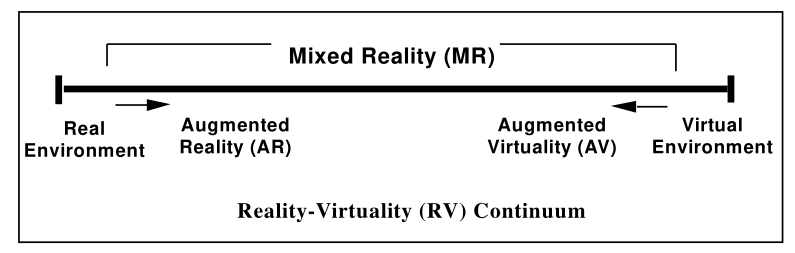
\includegraphics[keepaspectratio, width=\textwidth]{MR_milgram.png}
	\caption{Simplified representation of a RV continuum \parencite{Milgram1994}}
	\label{fig:RVContiinum}
\end{figure}

Fünf Jahre nach Milgram veröffentlichten \citeauthor{Kato1999} ihre Ergebnisse zu einem Marker-basierten AR Konferenzsystem. Sie lösten dabei das Problem der Registrierung (wo befindet sich der Benutzer, oder besser gesagt dessen Augen), und das Ermitteln der Pose (wie ist die Orientierung der virtuellen Kamera in Bezug zur Umwelt) über Marker mit einer fixen Grösse \parencite{Kato1999}. Das System war stationär mit Computern realisiert. In den folgenden Jahren wurden Versuche mit  mobilen Prototypen durchgeführt, dies blieben jedoch in der Grösse von Rucksäcken und gebrauchten Notebooks mit der entsprechenden Rechenleistung.

Ein grosser Durchbruch wurde deshalb von \citeauthor{Klein2009} erbracht, welche einen PTAM (Parallel Tracking and Mapping) Algorithmus auf einem iPhone 3G implementierten. Dieser war in der Lage sowohl in Räumen wie ausserhalb von Gebäuden, nach einer Initialisierungsphase die Lokalisierung von einem Marker loszulösen und die Pose der Kamera über \textquotedblleft Key Features\textquotedblright\ zu ermitteln \parencite{Klein2009}. Seither wurde auf diesem Gebiet weiter entwickelt und Algorithmen dieser Art sind unter dem Namen SLAM (Simultaneous Location and Mapping) zusammengefasst, dazu existieren verschiedene Frameworks welche diese nativ mitbringen (Kudan, wikitude).

\subsection{Konzepte}

\subsubsection{Markerbasierte Initialisierung}
Ein wichtiges Problem, das jede AR Appplikation lösen muss, ist die Registration. Damit ist gemeint, dass die Applikation Koordinatensysteme und Ausrichtung der virtuellen Welt mit der realen Welt abgleichen und überwachen muss.

Optische (d.h. Analyse der Kameradaten) Methoden werden von den gängigen Frameworks von Grund auf unterstützt. Zu diesen optischen Methoden gehören auch Marker. Ein Marker ist in den besten Fällen ein selbst unter Rotation und Scherung verformtes, eindeutig identifizierbares Muster, kann aber im Prinzip jegliches Bild sein. Ein guter Marker hat vorzugsweise einen hohen Kontrast im Grauspektrum, und grosse, komplexe Elemente ohne feine Details (welche auf Distanz verschwimmen oder verloren gehen) \cite{Kudan2016}.

Die eigentliche Erkennung der Marker geschieht mit Algorithmen der Computer Vision (Kantenerkennung, Eckenerkennung), worauf ein erkannter Marker mit einer Datenbank von bekannten abgeglichen wird. Danach kann über jenen einzelnen Marker sowohl Positionierung wie auch Lokalisation geschehen.

\subsubsection{SLAM}
Tracking-Methoden welche auf Marker basieren sind darauf angewiesen, dass jener zu jeder Zeit im Bild bleibt. Ansonsten verliert die Applikation dessen Registrierung. Eine andere Möglichkeit ist, ebenfalls mit Computer Vision, Feature-Points (ein Bildpunkt der sich durch seine lokale detaillierte Umgebung von anderen Punkten desselben Bilds hervorhebt) zu identifizieren (Location) und deren Abhängigkeiten zueinander in einer Karte zusammenfassen (Mapping). Sollte nun die Pose verloren werden (durch einen Unterbruch des Kamerastreams oder zu schnelle Bewegungen), muss nur ein Teil der vorherigen Karte wiedergefunden werden um die Position zu bestimmen.

\section{Anwendungen}

% TODO Industrie AR

% TODO Games

% TODO BIM

Auch im Bereich des BIM (Building Information Modelling) wurde im Zuge der Fortschritte in AR verschieden Lösungen erarbeitet. Neben spezialisierten Fachlösungen wie beispielsweise die DAQRI Smart Glasses (welche für AR und BIM im Industrieumfeld eingesetzt werden) \parencite{DAQRI2018}, wurde auch im wissenschaftlichen Umfeld interessante Prototypen entwickelt. So beispielsweise das Auto AR \parencite{Opperman2015} welche einem Benutzer erlaubt Neu- und geplante Bauten aus einem Auto zu begutachten, oder eine selbstentwickeltes BIM Framework des Frauenhofer Institut in Darmstadt \parencite{Olbrich2013}. Dennoch sind die Systeme von spezialisierter Hardware (GPS Sensoren, Serverbackend für Berechnungen) abhängig. Das Ziel unserer Arbeit soll sein BIM mittels einer AR Lösung auf handelsübliche Geräte (Smartphones, Tablets) zu bringen.

\chapter{Ideen und Konzepte}

\chapter{Methode}

\section{Vorgehensmodell}
% Beschreibung der agilen Projektmethode

\section{Anforderungsanalyse}

\section{Systemarchitektur}

\section{Komponentendesign}

\section{Umsetzung Programmierung}

\section{Testing}

\subsection{Testplan}

\subsection{Testfälle}

\chapter{Realisierung}

% TODO Ein Beispiel für den Gebrauch von Formeln und Referenz auf die jeweilige Formel - entfernen wenn nicht mehr gebraucht
Die Distanz zwischen zwei Geopositionen wird über die Bogenlänge (siehe \ref{Bogenlaenge}) der Differenz der Längen- und Breitengrade ausgerechnet.

\indexequation{b = \frac{\pi}{\SI{180}{\degree}}\beta r}{Bogenlänge des Winkels $\beta$ mit Radius $r$}{Bogenlaenge}

\subsection{Evaluation}
Im Rahmen dieses Projektes mussten verschiedene Unbekannte zuerst analysiert und evaluiert werden. Dazu ghörten die Zielplatform, Entwicklungsumgebung und die zu verwenden Augmented Reality Frameworks.
\subsubsection{Zielplattform}
Als Zielplatform standen gemäs Projektbeschrieb folgende zur Auswahl:
\begin{itemize}
\item Microsoft Hololens
\item Smartphone und Tablets
\end{itemize}
Für alle dieser Platformen galt die Idee, diese als Interface zu gebrauchen um das AR Gebäude in der Umgebung anzuzeigen. Alle drei Zielplattformen weisen unterschiedliche Stärken und Schwächen auf.



Die Hololens zeigte grosse Schwächen beim Gebrauch im Freien, da der Bildschirm in der Hololens für den Aussengebrauch zu wenig Hell ist. Zudem fehlen der Hololens Localisierungs Sensoren. In enem Blindtest mit Probanden welche die Hololens noch nicht trugen, zeigte sich, dass deren bedienung nicht intuitiv ist.
Das Positive an der Hololens ist die Nahtlose integration der Augmented Reality Modelle in die Umgebung des Betrachters.


??Zudem stellt sich bei der Entwicklung einer Software auf dieser Platform noch das Problem, dass für unser Projekt nur eine Hololens zur verfügung steht, was unweigerlich dazu führt, dass die Entwicklung an ein Ort gebunden ist.??
 
 
 
Die Smartphones Zeigen eine Grosse Stärke in der Verbreitung. Dies führt zu einer hohen vertrautheit des Benutzers mit dem Device. Zudem sind die Heutigen Smartphones auch hell genug um das Display bei normalen Tageslicht zu sehen.
Nachteile zeigen sich schliesslich in der Haltung des Gerätes, da für die einbindung der Augmented Reality modelle das Smartphone ständig in den Händen gehalten werden muss. 

Dank der Höheren verbreitung und der damit entstehenden höheren flexibilität beim entwickeln, viel die Entscheidung auf eine Smartphone lösung. Bedingt durch das vorhandene Knowlege im Team wurde dabei die Platform Android als Primäre Zielplatform selektiert.
\subsubsection{Entwicklungsumgebung}
Bedingt durch die Selektion der Zielplatform standen verschiedene Entwicklungsumgebungen zur verfügung. Dabei wurden folgende 2 Entwicklungsumgebungen Evauliert:
\begin{itemize}
\item Unity
\item AndroidStudio
\end{itemize}

Beide Platformen weissen Stärken und Schwächen auf. Um beide Entwicklungsumgebungen richtig zu Evaluieren wurden auf beiden kleine Prototypen getestet. Dabei entstand die folgende Auffassung.

Bei Unity ist das Erstellen einer ersten Lauffähigen Version sehr einfach. Ein weiterere Vorteil ist die Graphische darstellung der 3D modelle. Zudem würde eine Allfällige Portierung auf eine Andere Platform sehr einfach möglich sein. Bei der Entwicklung stellte sich jedoch heraus, dass Unity seine Schwächen mit den Sensoren von Android aufweisst. So wurden Localisation Sensor Daten nicht korrekt bis gar nicht Übermittelt. Zudem fehlte eine Zureichende Debug möglichkeit.

Bei Android Studio zeigte sich seine Stärke in den Debug möglichkeit und der Ausgezeichneten API Dokumentation. So funktionierten alle Sensoren beim ersten versuch. Die Schwächen dieser Entwicklungumgebung liegt darin, dass eine allfällige Portierung auf ein Anderes Device nur durch eine Neuimplementation möglich ist. Zudem werden die 3D Modelle nicht Dargestellt und müssen mit einer anderen Software Manipuliert werden.

Die unzureichende Debugmöglichkeiten sowie die problemen mit den Sensoren waren die Hauptgründe die Unity Entwicklungsumgebung nicht für die Implementation zu gebrauchen.

\subsubsection{Augmented Reality Frameworks}
Was wird Evaluirt?
In unsere recherche stellte sich heraus, dass es insgesammt 3 Gängige AR Frameworks gibt, welche unseren Anforderungen entsprechen.
Dazu zählen Kudan, Wikitude und Vuforia.
Vuforia weist die Stärke im Markerbased tracking auf, kann jedoch nicht mit SLAM punkten. Deshalb viel die ängere wahl auf Wikitude und Kudan. Da das interne Knowhow von Kuden schon etwas auf dem besseren Stand war, entschieden wir uns schliesslich Kudan als unser Framework zu verwenden.


Beschreiben wieso wir uns auf die Androidplattform beschränkt haben, dabei darf auch auf die Evaluation eingeganen werden


\subsection{Evaluation Entwicklungsumgebung}

\section{Einschränkungen und Abgrenzungen}
Wir haben uns selber von Crossplatform auf native android entwicklung eingeschränkt. Dies wie aus der Evaluation ersichtlich ist.
Weiter haben wir eine Android abwärtskompatibilität auf version 6.0 begränzt dies entspricht ca. 80\% aller Android besitzer. Der vorteil ist, dass wir neuere features wie das Abfragen der Permissions nicht weiter abwärtskompatibel gestallten müssen.
Zudem muss das Android Gerät folgende Systemanforderungen aufweisen:
	GyroSensor
	Location Sensor (GPS, GLOSNASS, GALILEO, BEIDU usw.)
	PPCompass??


\section{Projektmanagementplan}

\subsection{Projektorganisation}
Da beide Projektmitglieder ihre Kompetenzen eher in den technischen Bereichen dieses Projekts sehen, wurde von einer strikten Aufgabenteilung abgesehen.

Es wurde dennoch darauf geachtet, dass beide Mitglieder klare Verantwortungen übernehmen. Diese waren jedoch mehr in einer überwachenden Funktion gesehen, und soll nicht heissen, dass dieses Mitglied die Arbeit alleine leistete.

\vspace{1em}

\begin{tabularx}{\textwidth}{|X|X|}
	\hline
	\textbf{Teammitglied} & \textbf{Funktionen} \\
	\hline
	Pascal Baumann & \tabitem Dokumentation \\
	& \tabitem Testplanung \& Durchführung \\
	& \tabitem Projektmanagement \\
	\hline
	Dane Wicki & \tabitem Architektur \\
	& \tabitem Plattformanalyse \\
	\hline
\end{tabularx}

\newpage
\subsection{Projektführung}

\subsection{Rahmenplan}

Das Projekt wurde in 6 zweiwöchige Sprints unterteilt und in diesen iterativ entwickelt.

\vspace{1em}

\begin{figure}[h!]
	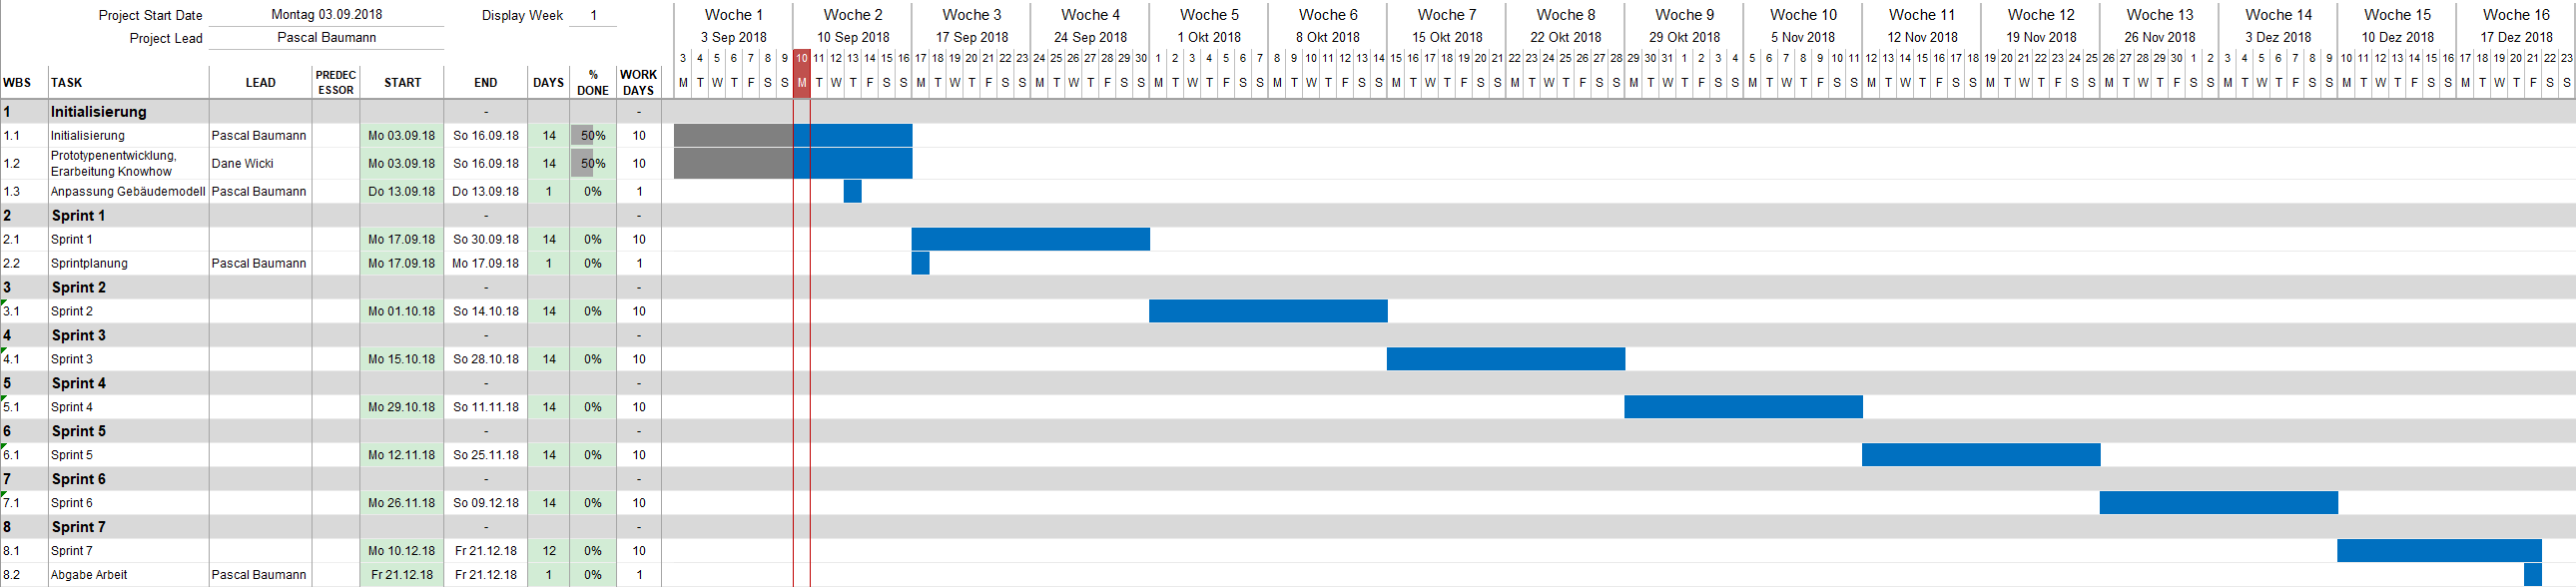
\includegraphics[keepaspectratio, width=\textwidth]{Rahmenplan}
	\caption{Überblick der Sprints}
\end{figure}

\subsection{Tools}
\label{sec:Tools}
\begin{table}[h!]
	\begin{tabular}{|p{0.4\textwidth}|p{0.6\textwidth}|}
		\hline
		\textbf{Aufgabe} & \textbf{Hilfsmittel} \\
		\hline
		Dokumente und Dokumentation & TeX / GitHub \\
		\hline
		Versionierung Dokumentation & git / GitHub\\
		\hline
		Dokumentation Code & JavaDoc \\
		\hline
		Git Clients & GitKraken, git Terminal\\
		\hline
		Quellen & Mendeley \\
		\hline
		Dateiablage für Teamaustausch & OneDrive \\
		\hline
		Rahmenplan & MS Excel 2016 \\
		\hline
		Kommunikation Team & WhatsApp\\
		\hline
		Aufgabenverwaltung & Trello, Rahmenplan\\
		\hline
		Entwicklungsumgebung Arduino & Arduino Studio\\
		\hline
	\end{tabular}
	\caption{Gebrauchte Software Hilfsmittel}
	\label{tab:SWTools}
\end{table}

\subsection{Risikomanagement}

Es werden mögliche Risiken welche während dem Projekt auftreten können aufgezählt. Diese werden auf Eintrittswahrscheinlichkeit und Schadensmass eingeschätzt, danach wird entschieden, welche Massnahmen getroffen werden können, und was deren Auswirkungen sind.

\subsubsection{Definitionen}
\label{sssec:Def}
\vspace{1em}
\noindent
Eintrittswahrscheinlichkeit:

\vspace{1em}
\noindent
\begin{tabular}{|p{0.06\textwidth}|p{0.2\textwidth}|p{0.7\textwidth}|}
	\hline
	\textbf{Stufe} & \textbf{Bezeichnung} & \textbf{Beschreibung} \\
	\hline
	1 & unvorstellbar & Möglich aber eher unwahrscheinlich. Tritt nie oder einmal in 14 Wochen auf \\
	\hline
	2 & unwahrscheinlich & Kann in 14 Wochen 1-5 Mal eintreten\\
	\hline
	3 & vorstellbar & Kann in 14 Wochen 6-8 Mal eintreten \\
	\hline
	4 & wahrscheinlich & Kann in 14 Wochen bis zu 10 Mal eintreten \\
	\hline
	5 & häufig & Kann in 14 Wochen 14 Mal eintreten\\
	\hline
\end{tabular}

\vspace{1em}
\noindent
Schadensausmass:

\vspace{1em}
\noindent
\begin{tabular}{|p{0.06\textwidth}|p{0.2\textwidth}|p{0.7\textwidth}|}
	\hline
	\textbf{Stufe} & \textbf{Bezeichnung} & \textbf{Beschreibung} \\
	\hline
	1 & unwesentlich & Die Aufgabenerfüllung wird höchstens geringfügig beeinträchtigt finanzieller Schaden ist im Rahmen des Projekts nicht beeinflussend. Personenschäden treten nicht auf \\
	\hline
	2 & geringfügig & Wahrnehmbare Gefährdung / Einfluss auf das Projekt. Personenschäden treten nicht auf \\
	\hline
	3 & mittelmässig & Wahrnehmbare Gefährdung / Einfluss auf das Projekt.Finanzieller Schaden strapaziert das Projektbudget
	Personenschäden treten nicht auf \\
	\hline
	4 & kritisch & Starke Gefährdung des Projekts. Finanzieller Schaden übersteigt das Projektbudget massiv. Personenschäden treten geringfügig auf \\
	\hline
	5 & katastrophal & Projektabbruch zur Folge. Finanzieller Schaden kann zum Projektstopp führen. Verletzung der Persönlichkeitsrechte
	\\
	\hline
\end{tabular}

\subsubsection{Risikokatalog}
\label{sssec:Risikokatalog}
Legende:
\begin{itemize}
	\item \textbf{S}chadensausmass bei Eintreffen des Risikos
	\item \textbf{W}ahrscheinlichkeit das Risiko eintrifft
	\item \textbf{K}ategorie: \textbf{T}echnisches oder \textbf{P}rojektbezogenes Risiko
	\item \textbf{A}uswirkung auf das Projekt. Produkt aus S und W
\end{itemize}

\vspace{1em}
\noindent
\begin{tabular}{|p{0.03\textwidth}|p{0.75\textwidth}|p{0.03\textwidth}|p{0.03\textwidth}|p{0.03\textwidth}||p{0.03\textwidth}|}
	\hline
	\textbf{Nr.} & \textbf{Beschreibung / Risiko} & \textbf{K} & \textbf{S} & \textbf{W} & \textbf{A} \\
	\hline
	1 & Datenverlust & P & 5 & 1 & 5\\
	\hline
	2 & Fehlkommunikation im Team & P & 3 & 2 & 6 \\
	\hline
	3 & Teammitglied fällt aus & P & 3 & 2 & 6 \\
	\hline
	4 & Verzug bei Erstellung von Dokumenten & P & 3 & 2 & 6 \\
	\hline
	5 & Prototyp entspricht nicht den Kundenwünschen & T & 5 & 2 & 10 \\
	\hline
\end{tabular}

\vspace{1em}

\begin{figure}[h!]
	\centering
	\includegraphics[keepaspectratio, width=0.8\textwidth]{Risikomatrix}
	\caption{Auswirkungen der Risiken}
\end{figure}

\section{Systemspezifikation}

\subsection{Systemübersicht}

\subsection{Architektur \& Design}

\subsection{Schnittstellen}

\subsection{Anforderungen}

\subsection{Anwendung}

\chapter{Evaluation und Validation}




\chapter{Ausblick}

\appendix

\chapter{Testprotokolle}


\glossary{Abkürzungsverzeichnis}

\listoffigures

\listoftables

\listofmyequations \pagebreak

\printbibliography

\chapter*{Eidesstattliche Erklärung}
Ich erkläre hiermit, dass ich/wir die vorliegende Arbeit selbständig und ohne unerlaubte fremde Hilfe angefertigt haben, alle verwendeten Quellen, Literatur und andere Hilfsmittel angegeben haben, wörtlich oder inhaltlich entnommene Stellen als solche kenntlich gemacht haben, das Vertraulichkeitsinteresse des Auftraggebers wahren und die Urheberrechtsbestimmungen der Fachhochschule Zentralschweiz (siehe Merkblatt «Studentische Arbeiten» auf MyCampus) respektieren werden.

\vspace{1em}

\renewcommand{\arraystretch}{2}
\begin{tabularx}{\textwidth}{XXXX}
	Unterschrift: & & Unterschrift: & \\ \cline{2-2}\cline{4-4}
	Baumann, Pascal & & Wicki, Dane & \\
	Datum: & & Ort: & \\
\end{tabularx}

\end{document}